\documentclass[10pt]{article}
\usepackage{graphicx, verbatim}
\usepackage{amsmath}
\usepackage{amssymb}
\usepackage{amscd}
\usepackage{lipsum}
\usepackage{todonotes}
\usepackage[tableposition=top]{caption}
%\usepackage{ifthen}texworks 
\usepackage[utf8]{inputenc}
\usepackage{graphicx}
\usepackage{caption}
\setlength{\textwidth}{6.5in} 
\setlength{\textheight}{9in}
\setlength{\oddsidemargin}{0in} 
\setlength{\evensidemargin}{0in}
\setlength{\topmargin}{-1.5cm}
\setlength{\parindent}{0cm}
\usepackage{setspace}
\usepackage{float}
\usepackage{amssymb}
\usepackage[utf8]{inputenc}
\usepackage{fancyhdr}
\usepackage{tabularx}
\usepackage{enumitem}
\usepackage{verbatim}
\usepackage{natbib}

\def\bibfont{\scriptsize}
\setlength{\bibsep}{0pt plus 0.3ex}

\usepackage{hyperref}
\hypersetup{
  colorlinks   = true, %Colours links instead of ugly boxes
  urlcolor     = blue, %Colour for external hyperlinks
  linkcolor    = blue, %Colour of internal links
  citecolor   = red %Colour of citations
}

%\fancyhf{}
\rfoot{Your Name \thepage}
\singlespacing
\usepackage[affil-it]{authblk} 
\usepackage{etoolbox}
\usepackage{lmodern}

\usepackage{titling}

\setlength{\droptitle}{-9em}

% Notice the following package, it will help you cite papers
%\usepackage[backend=bibtex ,sorting=none]{biblatex}
%\bibliography{references}

%\begin{filecontents*}{references.bib}

%\end{filecontents*}

%\AtBeginBibliography{\scriptsize}

\begin{document}

\font\myfont=cmr12 at 14pt
\title{{\myfont Part 1 -  Design Document for RGU Course Database }}
\author{\vspace{-10ex}}
\date{\vspace{-10ex}}
\maketitle
\vspace{-1cm}


\section{Introduction}
% The very first letter is a 2 line initial drop letter followed
% by the rest of the first word in caps.
% 
% form to use if the first word consists of a single letter:
% \IEEEPARstart{A}{demo} file is ....
% 
% form to use if you need the single drop letter followed by
% normal text (unknown if ever used by the IEEE):
% \IEEEPARstart{A}{}demo file is ....
% 
% Some journals put the first two words in caps:
% \IEEEPARstart{T}{his demo} file is ....
% 
% Here we have the typical use of a "T" for an initial drop letter
% and "HIS" in caps to complete the first word.
Prior to designing the database for the RGU course data, the following requirements were stated:
\begin{enumerate}
\item  \textit{Scalability}. It must be possible to add new courses, staff and student cohorts to the existing schema without altering the overall graph structure. In practice, this would be achieved by adding additional nodes.
\item \textit{Addition of new data}. Along with adding new properties, it should be possible to add new data to the existing schema. The given use case was to add data for new academic years.
\end{enumerate}
The briefing for the design was quite high level so a conservative approach was taken for design, as such the following principles and assumptions were identified:
\begin{enumerate}[label=\Alph*]
\item \textit{Minimise data redundancy}. Unlike a relational database, it is not necessarily practical/possible to normalise the data, but redundancy should be as low as possible without disproportionately affecting the other criteria.
\item \textit{ Maximise readability}. As the final user of the database was not specified, it is assumed it will be accessed by individuals with varying levels of experience (a well-designed database is generally more readable anyway). 
\item It must be possible to change any foreseeable attribute, and to add data for future academic years.

\end{enumerate}

\section{Design Choice}
The above considered, two overall designs were devised.

\subsection{Design 1 (discounted)}

\begin{figure}[h]
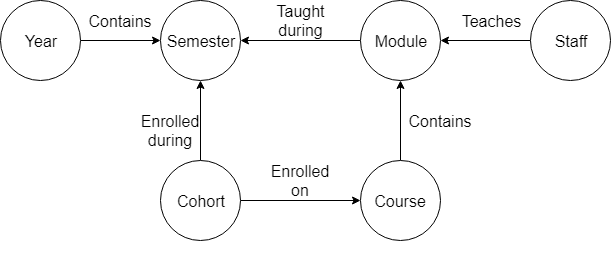
\includegraphics[scale=0.35]{design2}
\centering
\caption{Low relationship but high node-count design with normalised time properties}
\end{figure}

This design echoes the principles of relational database design and attempts to normalise the date-related properties with a timeline tree \citep{graphDBs} so ensures date entries do not need to be repeatedly entered when new data is added. This however, comes at the expense of ‘node redundancy’. Each node would require duplication in this model as new data is added. For example if module ‘M1’ was taught during semester 1 for course ‘C1, and semester 2 for course ‘C2’, the database would contain this subgraph: 

\begin{figure}[h]
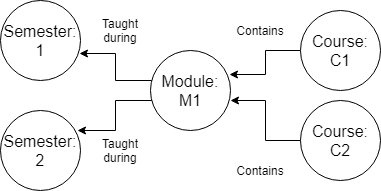
\includegraphics[scale=0.35]{subgraph}
\centering
\caption{subgraph from design 1 showing the need for either duplicate nodes or date-related relationship attributes}

\end{figure}

In this case, it is impossible to identify which course receives teaching for the module on a given semester without adding date attributes to the relationships. This completely negates the need for a timeline tree. Furthermore the requirement to duplicate nodes goes against the principle of minimising redundency. Adding a new year to this database would likely require a duplicate version of many nodes (essentially re-loading the database for every new year).

\subsection{Design 2 (Adopted for the final design)}

The full data model is shown in Figure \ref{modelf}.
\begin{figure}[h]
\centering
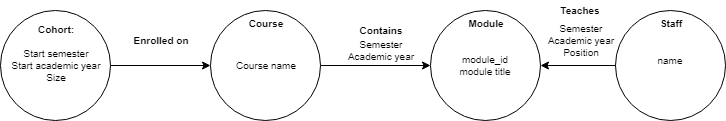
\includegraphics[scale=0.65]{full_design}
\caption{Design of the proposed model}
\label{modelf}

\end{figure}

Unlike the previous option which would have a high node-count, this graph has a high relationship count. Although this leads to duplicated time data, it allows for any nodes to be re-mapped to any other eligible node as teaching schedules/course agendas change over time by adding new relationships.This design meets the requirements/principles outlined in the introduction as follows:

\textit{Mandatory criteria}\\
\begin{enumerate}

\item It is relatively simple to add a new course, module or staff member. They are simply added as a new node and only need to be added once (ie they do not require separate entries for every academic year). The associated relationships can then be entered to link nodes up.
\item Adding data for a new academic year is achieved by simply adding new relationships between the existing nodes. This maintains a simpler graph with fewer nodes at the cost of having to re-enter the year and semester every time a new relationship is created.
For example, if Ines Arana continues to teach CMM510 in the 2018 academic year, we need to add a relationship to record thus:


%\texttt{
\begin{verbatim}
 MATCH(s:Staff{name:'Ines Arana'}),(m:Module{module_id:'CMM510'}) 
\end{verbatim}
\begin{verbatim}
CREATE (s)-[:teaches{position:'course_leader',academic_year:2018}]->(m)
\end{verbatim}
%}
This adds a 'teaches' relationship for 2018 between the nodes:
\begin{figure}[h]
\centering
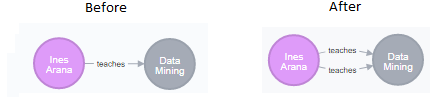
\includegraphics[scale=1]{change}
\caption{Example result of adding data for a new academic year}

\end{figure}

Adding new relationships in this manner does not re-structure the graph as a whole. This means data for a new year can be added on an ad-hoc basis and queries written at one point in time will continue to work in the future. 
The exception is for the ‘Cohort’ node which requires new nodes for every academic year. This is necessary since cohorts are unique to academic year.
\end{enumerate}

\textit{Other design principles}
\begin{enumerate}[label=\Alph*]
\item ‘Year’ and ‘semester’ entries are stored multiple times. This was a necessary compromise to allow all the nodes to contain unique data only.
\item The above decision reduced the node count and makes for a simpler graph overall. It should be noted that a .grass stylesheet is also included with the final design to help improve readability.
\item It is possible to update any combination of course/staff/modules in the given design (cohort is immutable since they are only defined once at the time of enrolment).
\end{enumerate}

\newpage








%
% paper title
% Titles are generally capitalized except for words such as a, an, and, as,
% at, but, by, for, in, nor, of, on, or, the, to and up, which are usually
% not capitalized unless they are the first or last word of the title.
% Linebreaks \\ can be used within to get better formatting as desired.
% Do not put math or special symbols in the title.
\font\myfont=cmr12 at 14pt
\title{{\myfont Part 2 - A Technical Comparison of Apache HBase and Cassandra }}
\author{\vspace{-10ex}}
\date{\vspace{-10ex}}
\maketitle
\vspace{-1cm}
%





\section{Introduction}
Apache HBase and Cassandra are superficially similar databases; both following the wide-column model and being based on preceding BigTable databases. Both were initially released in 2008 and have seen widespread use from commercial and academic users in the subsequent decade and they remain a popular alternative to relational database management systems (RDBMS).

\section{General Architecture}
\subsection {HBase Architecture}
HBase may be considered one of the components of the Hadoop ecosystem. It runs on top of the HDFS filesystem, and so may be used to store and retrieve data with all the advantages of HDFS, but also allowing for fast data access as HBase is optimised to allow for multiple random reading and writing of data, rather than the 'write once read many times' use case that HDFS is typically used for.  Hbase stores data in HDFS files, which are split between 'region servers', these act on top of HDFS data nodes - with the number of region servers being equal to the number of HDFS nodes available. The region servers are controlled by master servers which update individual tables in the region servers as required \citep{6885425}. Zookeeper, whch is part of the standard Hadoop stack, acts to control the entire cluster, monitoring the region and master servers; therefore allowing for load balancing and node failure detection. A weakness with this setup is that a namenode is required which can form a single point of failure if a hot standby type configuration is not utilised.\\

The structure of HBase tables themselves is derived from Google's BigTable database. Hbase is a column orientated database and, as such, is designed to store structured data (or at least, semi structured data). Each table is divided into column families, with each column family comprising of multiple columns. Each row requires a key - allowing for unique rows to be identified. Crucially, columns are not saved in a fixed schema; only column families are defined. This allows for dynamic scaling of tables in the 'width' direction, allowing HBase to achieve its design goal of tables on the order of 'billions of rows and millions of columns'. Tables are automatically sharded between the available HDFS nodes \citep{hbaseref}.\\

In order to account for high write-demand applications, HBase makes use of Log-Structures Merge Trees (LSMTs)  \citep{hbaseref}. Each update is first written to the Write Ahead Log (present for every region server). For each table partition affected by the update the Memstore, which is an in-memory tree, is updated. The memstore is periodically written to HFiles,  which are immutable and reside on the disk, as the memory limit is exceeded. Bloom filters may be enabled in order to reduce the number of disk accesses.\\

\subsection{Cassandra Architecture}
Cassandra operates independantly of HDFS, using it's own file system - CFS. This means the filesystem is not constrained by the existing architecture of HDFS. Like HBase, Cassandra splits data between multiple nodes in a cluster. However, unlike HBase, each node is identical in structure and purpose. Every second all nodes exchange information with every other node to ensure data is consistent across the entire cluster. This ensures that, providing nodes are located in seperate physical locations, Cassandra under no circumstances has a single failure point. Every node contains a commit log, which is modified every time the node performs a write or update. The high level of distribution and consistent, homogeneous nature of individual nodes makes Cassandra ideal for deployment in multiple locations where it can operate in an 'always on' manner \citep{cassandraarch}.\\

Tables in Cassandra differ from HBase in that they are modelled after DynamoDB. Fundementally, the struture of a table is similar to HBase, with each table consisting of a number of column families, each of which contain a number of columns \citep{7507964}. It is helpful not to think of a Cassandra database as a collection of tables split into columns. Rather, each column family is more analogous to a table in a RDB; within each column family, the columns are arranged in a nested sorted map which allows for a huge number of columns to be stored and retrieved. Each cell is identified by a unique row and column key. Since the number of column keys is unbounded, and columns can be valueless, the format of columns is variable; making Cassandra a wide column database, like HBase. \citep{harrison}\\

At the node level, data writes in Cassandra are similar to HBase. Each write is written to the commit log and then to the memtable where it is indexed in memory. The subsequent use of LSMTs, along with a sequentially updated commit log and periodic consolidation of immutable on-disk structures, make Casandra and HBase structurally similar at the node level.

\section{Features Comparison}
In order to compare the advantages of each database, the constituents of CAP theorem are considered \citep{harrison}.
In addition, read write performance of each database is also compared. One of the desirable features of NoSQL databases is the ability to run fast write/read operations for applicable use cases, so the performance is crucial when comparing databases.

\subsection{CAP Overview}
It is impossible to guarantee all three facets of CAP in a distributed database, so systems are typically designed on a 'pick two' philosophy. Cassandra and HBase differ in this respect, in that Cassandra is optimised for Partition Tolerance and Availability (AP) while HBase is optimised for Consistency and Partition-Tolerance (CP). For reference, RDBMS systems typically guarantee Consistency and Availability (CA) at the cost of partition tolerance\citep{harrison}.

\subsection{Consistency}
HBase guarantees consistency by first guaranteeing Atomicity. This means any change (mutation) to a row either occurs in entirity or not at all, so it is not possible to partially update a given row. As a result, any row returned by a query is guaranteed to be a complete row that existed at some point in the table history. HBase strictly enforces strong consistency, and as such this requirment is not tuneable. Cassandra does not guarantee consistency, as it is constrained to eventual consistency only, but the level of consistency is tuneable at the expense of availability. Previous tests have shown the inconsistency window following a request to be relativley short, even under high workload; although if the system is places under sufficient computational stress, consistency becomes unpredictable. \citep{10.1007/978-3-319-04936-6_3}

\subsection{Availability}
HBase sacrifices availability for Consistency and is therefore typically not used for the realtime streaming applications that Cassandra is used for. The reduced availability of HBase stems from the use of region servers. The loss of a region server causes availability to be degraded until other servers can be reassigned. This loss of availability actually guarantees consistency, since all users can only access a single version of the data \citep{6885425}. Cassandra, on the other hand, is designed to ensure high availability. This is achieved through the consistent structure of each node so if a node goes offline the commit log from other nodes may be used to provide access to the data immediately. The drawback of this high availability is that there is no guarantee all nodes will be in sync at the time of the request, so consistency is not guaranteed. However, unlike HBase, Casssandra allows the user to manually set the level of availability, and corresponding loss of consistency. Due to this tuning ability, Cassandra doesnt sit firmly in one corner of the CAP triangle, although it cannot guarantee the same level of consistency as HBase.

\subsection{Partition Tolerance}
Running atop HDFS, HBase inherently has high partition tolerance. The use of Zookeeper to manage individual nodes ensures coordination between nodes and maintains a high level of redundancy across the entire cluster \citep{6846507}. Cassandra exhibits a similar level of partition tolerance to HBase; while it does not depend on HDFS, it runs its own independant protocol to ensure sufficient redundency between nodes \citep{DBLP:journals/corr/RahmanTNGV15}.

\subsection{Performance}
While both databases are designed to support fast random access to data, broadly speaking Cassandra is optimised for writing where HBase is optimised for reading. Multiple studies have observed significantly faster performance from Cassandra for read-intensive queries. Benchmark tests running locally on a virtual machine have showed Cassandra to be consistently faster at both reading and writing \citep{abrberfur2014}, with both query types requiring approximaely half the time for 1000 read operations over on the order of half a million rows. Subsequent tests on a local cluster gave similar results, with Cassandra exhibiting superior write performance as the database size was scaled up \citep{7507964}. Recent tests on a 4 node cluster indicated marginally better read performance for HBase for 100,000 records \citep{7979888}. While these tests again showed better write performance for Cassandra, the difference was lesser so than previous tests, with HBase capable of writing 100,000 records in ~4000ms, to Cassandra's time of ~5500ms. Cassandra was also shown to scale better as the record count increased, with HBase peaking in throughput at 100000 writes, while Cassandra's throughput in operations/second continued to increase with write count.\\

In reality, benchmark testing can only reveal so much about performance since the two databases are enterprise products used by commercial organisations. Although Cassandra generally outperforms HBase for both write and read operations \citep{DBLP:journals/corr/abs-1208-4167}, this is not necesaily true for all real-world use cases. When databases are scaled up, with nodes and end users seperated geographically, HBase has been shown to exhibit improved read-performance for multiple use-cases \citep{xu2017}.


\section{Conclusions}
In a hypothetical scenario where all things are equal, Cassandra would be chosen for applications requiring fast read and writes, but where consistency is not as much of a concern. HBase guarantees consistency to a greater extent than Cassandra, so would be chosen for use cases where this is important. Both are highly partition tolerant, a common feature for most NoSQL databases. In reality it is unreasonable to draw any firm conclusions since there is never a 'best' database - only one which is best suited for the use-case at hand.

% The very first letter is a 2 line initial drop letter followed
% by the rest of the first word in caps.
% 
% form to use if the first word consists of a single letter:
% \IEEEPARstart{A}{demo} file is ....
% 
% form to use if you need the single drop letter followed by
% normal text (unknown if ever used by the IEEE):
% \IEEEPARstart{A}{}demo file is ....
% 
% Some journals put the first two words in caps:
% \IEEEPARstart{T}{his demo} file is ....
% 
% Here we have the typical use of a "T" for an initial drop letter
% and "HIS" in caps to complete the first word.

% if have a single appendix:
%\appendix[Proof of the Zonklar Equations]
% or
%\appendix  % for no appendix heading
% do not use \section anymore after \appendix, only \section*
% is possibly needed

% use appendices with more than one appendix
% then use \section to start each appendix
% you must declare a \section before using any
% \subsection or using \label (\appendices by itself
% starts a section numbered zero.)
%


\bibliographystyle{agsm}
\bibliography{references}


%\bibliography{references}








% trigger a \newpage just before the given reference
% number - used to balance the columns on the last page
% adjust value as needed - may need to be readjusted if
% the document is modified later
%\IEEEtriggeratref{8}
% The "triggered" command can be changed if desired:
%\IEEEtriggercmd{\enlargethispage{-5in}}

% references section

% can use a bibliography generated by BibTeX as a .bbl file
% BibTeX documentation can be easily obtained at:
% http://mirror.ctan.org/biblio/bibtex/contrib/doc/
% The IEEEtran BibTeX style support page is at:
% http://www.michaelshell.org/tex/ieeetran/bibtex/
%\bibliographystyle{IEEEtran}
% argument is your BibTeX string definitions and bibliography database(s)
%\bibliography{IEEEabrv,../bib/paper}
%
% <OR> manually copy in the resultant .bbl file
% set second argument of \begin to the number of references
% (used to reserve space for the reference number labels box)


% biography section
% 
% If you have an EPS/PDF photo (graphicx package needed) extra braces are
% needed around the contents of the optional argument to biography to prevent
% the LaTeX parser from getting confused when it sees the complicated
% \includegraphics command within an optional argument. (You could create
% your own custom macro containing the \includegraphics command to make things
% simpler here.)
%\begin{IEEEbiography}[{\includegraphics[width=1in,height=1.25in,clip,keepaspectratio]{mshell}}]{Michael Shell}
% or if you just want to reserve a space for a photo:


% You can push biographies down or up by placing
% a \vfill before or after them. The appropriate
% use of \vfill depends on what kind of text is
% on the last page and whether or not the columns
% are being equalized.

%\vfill

% Can be used to pull up biographies so that the bottom of the last one
% is flush with the other column.
%\enlargethispage{-5in}



% that's all folks
\end{document}


